% Template Created by Albert Alises Sorribas (albert.alises@gmail.com) for the thesis of the MSc. in Computational Biomedical Engineering, Universitat Pompeu Fabra. Based on the thesis template of the Imperial College London,  downloadable at http://www.imperial.ac.uk/brand-style-guide/templates/downloadable-templates/

\documentclass[a4paper,12pt,twoside]{report}
\usepackage[left=3cm,right=3cm,top=3cm,bottom=3cm]{geometry} %Margins
\usepackage{pdfpages}
\usepackage{hyperref}
\usepackage{listings}
\usepackage{xcolor}
\usepackage{setspace}
\usepackage{tocloft}
\usepackage{amsmath}
\usepackage{chngcntr }
\usepackage[toc,page]{appendix}
\usepackage[T1]{fontenc}
\usepackage[nottoc]{tocbibind}
\usepackage[compact]{titlesec}
\titlespacing{\section}{0pt}{1ex}{0ex}
\titlespacing{\subsection}{0pt}{1ex}{0ex}
\titlespacing{\subsubsection}{0pt}{1ex}{0ex}

\counterwithout{figure}{chapter}
\counterwithout{table}{chapter}

\usepackage{graphicx}
\usepackage{verbatim}
\usepackage{latexsym}
\def\bbbr{{\rm I\!R}} %reelle Zahlen
\def\bbbm{{\rm I\!M}}
\def\bbbn{{\rm I\!N}} %natuerliche Zahlen
\def\bbbf{{\rm I\!F}}
\def\bbbh{{\rm I\!H}}
\def\bbbk{{\rm I\!K}}
\def\bbbp{{\rm I\!P}}
\def\bbbe{{\rm I\!E}}
\def\bbbone{{\mathchoice {\rm 1\mskip-4mu l} {\rm 1\mskip-4mu l}
{\rm 1\mskip-4.5mu l} {\rm 1\mskip-5mu l}}}
\def\bbbc{{\mathchoice {\setbox0=\hbox{$\displaystyle\rm C$}\hbox{\hbox
to0pt{\kern0.4\wd0\vrule height0.9\ht0\hss}\box0}}
{\setbox0=\hbox{$\textstyle\rm C$}\hbox{\hbox
to0pt{\kern0.4\wd0\vrule height0.9\ht0\hss}\box0}}
{\setbox0=\hbox{$\scriptstyle\rm C$}\hbox{\hbox
to0pt{\kern0.4\wd0\vrule height0.9\ht0\hss}\box0}}
{\setbox0=\hbox{$\scriptscriptstyle\rm C$}\hbox{\hbox
to0pt{\kern0.4\wd0\vrule height0.9\ht0\hss}\box0}}}}
\def\bbbq{{\mathchoice {\setbox0=\hbox{$\displaystyle\rm
Q$}\hbox{\raise
0.15\ht0\hbox to0pt{\kern0.4\wd0\vrule height0.8\ht0\hss}\box0}}
{\setbox0=\hbox{$\textstyle\rm Q$}\hbox{\raise
0.15\ht0\hbox to0pt{\kern0.4\wd0\vrule height0.8\ht0\hss}\box0}}
{\setbox0=\hbox{$\scriptstyle\rm Q$}\hbox{\raise
0.15\ht0\hbox to0pt{\kern0.4\wd0\vrule height0.7\ht0\hss}\box0}}
{\setbox0=\hbox{$\scriptscriptstyle\rm Q$}\hbox{\raise
0.15\ht0\hbox to0pt{\kern0.4\wd0\vrule height0.7\ht0\hss}\box0}}}}
\def\bbbt{{\mathchoice {\setbox0=\hbox{$\displaystyle\rm
T$}\hbox{\hbox to0pt{\kern0.3\wd0\vrule height0.9\ht0\hss}\box0}}
{\setbox0=\hbox{$\textstyle\rm T$}\hbox{\hbox
to0pt{\kern0.3\wd0\vrule height0.9\ht0\hss}\box0}}
{\setbox0=\hbox{$\scriptstyle\rm T$}\hbox{\hbox
to0pt{\kern0.3\wd0\vrule height0.9\ht0\hss}\box0}}
{\setbox0=\hbox{$\scriptscriptstyle\rm T$}\hbox{\hbox
to0pt{\kern0.3\wd0\vrule height0.9\ht0\hss}\box0}}}}
\def\bbbs{{\mathchoice
{\setbox0=\hbox{$\displaystyle     \rm S$}\hbox{\raise0.5\ht0\hbox
to0pt{\kern0.35\wd0\vrule height0.45\ht0\hss}\hbox
to0pt{\kern0.55\wd0\vrule height0.5\ht0\hss}\box0}}
{\setbox0=\hbox{$\textstyle        \rm S$}\hbox{\raise0.5\ht0\hbox
to0pt{\kern0.35\wd0\vrule height0.45\ht0\hss}\hbox
to0pt{\kern0.55\wd0\vrule height0.5\ht0\hss}\box0}}
{\setbox0=\hbox{$\scriptstyle      \rm S$}\hbox{\raise0.5\ht0\hbox
to0pt{\kern0.35\wd0\vrule height0.45\ht0\hss}\raise0.05\ht0\hbox
to0pt{\kern0.5\wd0\vrule height0.45\ht0\hss}\box0}}
{\setbox0=\hbox{$\scriptscriptstyle\rm S$}\hbox{\raise0.5\ht0\hbox
to0pt{\kern0.4\wd0\vrule height0.45\ht0\hss}\raise0.05\ht0\hbox
to0pt{\kern0.55\wd0\vrule height0.45\ht0\hss}\box0}}}}
\def\bbbz{{\mathchoice {\hbox{$\mathsf\textstyle Z\kern-0.4em Z$}}
{\hbox{$\mathsf\textstyle Z\kern-0.4em Z$}}
{\hbox{$\mathsf\scriptstyle Z\kern-0.3em Z$}}
{\hbox{$\mathsf\scriptscriptstyle Z\kern-0.2em Z$}}}}
\usepackage{setspace}
\usepackage{blindtext}
\usepackage{float}

\setlength{\parskip}{\medskipamount}  % a little space before a \par
\setlength{\parindent}{0pt}	      % don't indent first lines of paragraphs
%UHEAD.STY  If this is included after \documentstyle{report}, it adds
% an underlined heading style to the LaTeX report style.
% \pagestyle{uheadings} will put underlined headings at the top
% of each page. The right page headings are the Chapter titles and
% the left page titles are supplied by \def\lefthead{text}.

% Ted Shapin, Dec. 17, 1986

\makeatletter
\def\chapapp2{Chapter}

\def\appendix{\par
 \setcounter{chapter}{0}
 \setcounter{section}{0}
 \def\chapapp2{Appendix}
 \def\@chapapp{Appendix}
 \def\thechapter{\Alph{chapter}}}

\def\ps@uheadings{\let\@mkboth\markboth
% modifications
\def\@oddhead{\protect\underline{\protect\makebox[\textwidth][l]
		{\sl\rightmark\hfill\rm\thepage}}}
\def\@oddfoot{}
\def\@evenfoot{}
\def\@evenhead{\protect\underline{\protect\makebox[\textwidth][l]
		{\rm\thepage\hfill\sl\leftmark}}}
% end of modifications
\def\chaptermark##1{\markboth {\ifnum \c@secnumdepth >\m@ne
 \chapapp2\ \thechapter. \ \fi ##1}{}}%
\def\sectionmark##1{\markright {\ifnum \c@secnumdepth >\z@
   \thesection. \ \fi ##1}}}
\makeatother
%%From: marcel@cs.caltech.edu (Marcel van der Goot)
%%Newsgroups: comp.text.tex
%%Subject: illegal modification of boxit.sty
%%Date: 28 Feb 92 01:10:02 GMT
%%Organization: California Institute of Technology (CS dept)
%%Nntp-Posting-Host: andromeda.cs.caltech.edu
%%
%%
%%Quite some time ago I posted a file boxit.sty; maybe it made it
%%to some archives, although I don't recall submitting it. It defines
%%	\begin{boxit}
%%	...
%%	\end{boxit}
%%to draw a box around `...', where the `...' can contain other
%%environments (e.g., a verbatim environment). Unfortunately, it had
%%a problem: it did not work if you used it in paragraph mode, i.e., it
%%only worked if there was an empty line in front of \begin{boxit}.
%%Luckily, that is easily corrected.
%%
%%HOWEVER, apparently someone noticed the problem, tried to correct it,
%%and then distributed this modified version. That would be fine with me,
%%except that:
%%1. There was no note in the file about this modification, it only has my
%%   name in it.
%%2. The modification is wrong: now it only works if there is *no* empty
%%   line in front of \begin{boxit}. In my opinion this bug is worse than
%%   the original one.
%%
%%In particular, the author of this modification tried to force an empty
%%line by inserting a `\\' in the definition of \Beginboxit. If you have
%%a version of boxit.sty with a `\\', please delete it. If you have my
%%old version of boxit.sty, please also delete it. Below is an improved
%%version.
%%
%%Thanks to Joe Armstrong for drawing my attention to the bug and to the
%%illegal version.
%%
%%                                          Marcel van der Goot
%% .---------------------------------------------------------------
%% | Blauw de viooltjes,                    marcel@cs.caltech.edu
%% |    Rood zijn de rozen;
%% | Een rijm kan gezet
%% |    Met plaksel en dozen.
%% |


% boxit.sty
% version: 27 Feb 1992
%
% Defines a boxit environment, which draws lines around its contents.
% Usage:
%   \begin{boxit}
%	... (text you want to be boxed, can contain other environments)
%   \end{boxit}
%
% The width of the box is the width of the contents.
% The boxit* environment behaves the same, except that the box will be
% at least as wide as a normal paragraph.
%
% The reason for writing it this way (rather than with the \boxit#1 macro
% from the TeXbook), is that now you can box verbatim text, as in
%   \begin{boxit}
%   \begin{verbatim}
%   this better come out in boxed verbatim mode ...
%   \end{verbatim}
%   \end{boxit}
%
%						Marcel van der Goot
%						marcel@cs.caltech.edu
%

\def\Beginboxit
   {\par
    \vbox\bgroup
	   \hrule
	   \hbox\bgroup
		  \vrule \kern1.2pt %
		  \vbox\bgroup\kern1.2pt
   }

\def\Endboxit{%
			      \kern1.2pt
		       \egroup
		  \kern1.2pt\vrule
		\egroup
	   \hrule
	 \egroup
   }	

\newenvironment{boxit}{\Beginboxit}{\Endboxit}
\newenvironment{boxit*}{\Beginboxit\hbox to\hsize{}}{\Endboxit}
\pagestyle{empty}

\setlength{\parskip}{2ex plus 0.5ex minus 0.2ex}
\setlength{\parindent}{0pt}

\makeatletter  %to avoid error messages generated by "\@". Makes Latex treat "@" like a letter

\linespread{1.5}
\def\submitdate#1{\gdef\@submitdate{#1}}
\def\supervisor#1{\gdef\@supervisor{#1}}
\def\cosupervisor#1{\gdef\@cosupervisor{#1}}

\def\maketitle{
  % Title
  \begin{titlepage}{
    \vspace*{2\baselineskip} %Empty Lines
    {\fontsize{17.28}{16.8}\selectfont Master thesis Sound and Music Computing}\\
     {\fontsize{14}{16.8}\selectfont Universitat Pompeu Fabra}\\
    \rm
    \vspace*{3\baselineskip} %Empty Lines
     \bf \fontsize{24.88}{17.5}\selectfont  \@title \par
  }
  \vskip 0.3in
  \par
  {\fontsize{14}{27}\selectfont  \@author}

  \vskip 0.20in
  \fontsize{14}{16.8}\selectfont \textbf{Supervisor:}   \@supervisor \\
  \fontsize{14}{16.8}\selectfont \textbf{Co-Supervisor:}  \@cosupervisor \\
   \vspace*{3\baselineskip} %Empty Lines
    \fontsize{14}{27}\selectfont  \@submitdate \\
    \vspace{ 0.7in}
    
\includegraphics[width=8cm]{Figures/LogoPompeuFabra}\\[.5cm]
  \vfil
  \end{titlepage}
}

\def\titlepage{
  \newpage
  \centering
  \linespread{1.5}
  \normalsize
  \vbox to \vsize\bgroup\vbox to 9in\bgroup
}
\def\endtitlepage{
  \par
  \kern 0pt
  \egroup
  \vss
  \egroup
  \cleardoublepage
}

\def\abstract{
  \begin{center}{
    \large\bf Abstract}
  \end{center}
  \small
  %\def\baselinestretch{1.5}
  \linespread{1.5}
  \normalsize
}
\def\endabstract{
  \par
   \cleardoublepage
}

\newenvironment{acknowledgement}{
  \clearpage
  \begin{center}{
    \large \bf Acknowledgement}
  \end{center}
  \small
  \linespread{1.5}
  \normalsize
}{\clearpage}
\def\endacknowledgement{
  \par
    \cleardoublepage
}

\newenvironment{dedication}{
  \clearpage
  \begin{center}{
    \large \bf Dedication}
  \end{center}
  \small
  \linespread{1.5}
  \normalsize
}{\clearpage}
\def\enddedication{
  \par
  \cleardoublepage
}

\def\preface{
    \pagenumbering{gobble}
    \pagestyle{plain}
    \doublespacing
     \setcounter{tocdepth}{2}
    \tableofcontents
}

\def\body{

    \clearpage
    \pagestyle{uheadings}
    \pagenumbering{arabic}
    \singlespacing
    \setlength{\cftbeforesecskip}{10pt}

    \pagestyle{plain}
    \clearpage
    \pagestyle{uheadings}

}

\makeatother  %to avoid error messages generated by "\@". Makes Latex treat "@" like a letter


\newcommand{\titlelinespacing}{\renewcommand{\baselinestretch}{2.0} \normalsize}
\newcommand{\normallinespacing}{\renewcommand{\baselinestretch}{1.5} \normalsize}
\newcommand{\mediumlinespacing}{\renewcommand{\baselinestretch}{1.2} \normalsize}
\newcommand{\narrowlinespacing}{\renewcommand{\baselinestretch}{1.0} \normalsize}

\newtheorem{definition}{Definition}[chapter]
\newtheorem{theorem}{Theorem}[chapter]
\cftsetindents{section}{0in}{0.5in}
\cftsetindents{subsection}{0in}{0.5in}
\cftsetindents{subsubsection}{0in}{0.5in}
\cftsetindents{paragraph}{0in}{0.5in}


\begin{document}

\newgeometry{left=2cm,right=2cm} %Only for the title new margins

%Title parameters
\title{Automatic harmonic analysis of classical string quartets from symbolic score}
\author{N\'estor N\'apoles L\'opez}
\submitdate{September 2017}
\supervisor{Xavier Serra}
\cosupervisor{Rafael Caro}

\maketitle

\maketitle
\restoregeometry

\preface
\cleardoublepage
%\addcontentsline{toc}{chapter}{Acknowledgement}
\begin{dedication}
\pagenumbering{gobble}% Remove page numbers (and reset to 1)

Grandmother, Juan Rodrigo Perez Cardenas. Family. Kinga.

\newpage

\end{dedication}

%\addcontentsline{toc}{chapter}{Acknowledgement}

\begin{acknowledgement}
\pagenumbering{gobble}% Remove page numbers (and reset to 1)

Xavier Serra, I am thankful for the trust deposited in my music theory skills for performing this work, and for allowing me to contribute to the CompMusic project.

Rafael Caro, thank you for helping with the harmonic analyses and the fast review of every presentation and thesis draft.

Craig Sapp, thank you for the fast response in the topics related to Humdrum Extras, the Verovio Humdrum Viewer and for pointing out to relevant research I was unaware of. 

\newpage
\end{acknowledgement}

%\addcontentsline{toc}{chapter}{Abstract}

\begin{abstract}
\pagenumbering{gobble}

This work proposes running an automatic harmonic analysis over a novell dataset of String Quartets from Joseph Haydn. Using implementation code from David Temperley, Daniel Sleator and Craig Sapp. Additionally, proposes an evaluation method to measure the similarity of the resulting analyses against manual annotations included in the String Quartet dataset. 24 musical scores analyzed and evaluated with a range of 15\% to 85\% accuracy for the Temperley algorithm.

\bigskip
Keywords: Automatic harmonic analysis; Joseph Haydn; String quartet; Roman numeral analysis


\newpage
\end{abstract}


\body

\normallinespacing

% Introduction of the project
\chapter{Introduction}
In the traditional sense, harmonic analysis relates to a set of music theory studies that pretend to describe the relationship of simultaneous sonorities and generalize rules of how each of the voices involved should move to facilitate and embellish these simultaneous sonorities.

It is difficult, however, to give a precise definition of where the task of automatic harmonic analysis starts and finishes. As will be discussed in the literature review, different researchers have made different characterizations of the problem, sometimes binding these characterizations closely to the mathematical tools they have used to approach the problem, in other cases to the type of music that they pretend to analyze, and in other cases due to other circumstances. For this particular work, I intend to define harmonic analysis based in two simple definitions, and afterwards, the outcome definition will help to describe which are the expected inputs and outputs of an automatic harmonic analysis system.

\section{Harmonic analysis}
According to the Oxford Music Online dictionary, in the context of music, the term \emph{analysis} could be defined as the following: \cite{oxfordanalysis}

\begin{quote}
\centering
\emph{[...] the interpretation of structures in music, \linebreak
their resolution into relatively simpler constituent elements, \linebreak and the investigation of the relevant functions of those elements.}
\end{quote}

Additionally, according to the same source, a very simplistic definition of harmony could be: \cite{oxfordharmony}

\begin{quote}
\centering
\emph{The simultaneous sounding (i.e. combination) of notes [...]}
\end{quote}

\begin{figure}[h]
  \caption{Excerpt from Joseph Haydn's Op.20 No.3 - II. Menuetto: Allegretto, mm. 1-6}
  \label{fig:harmony}
  \centering
    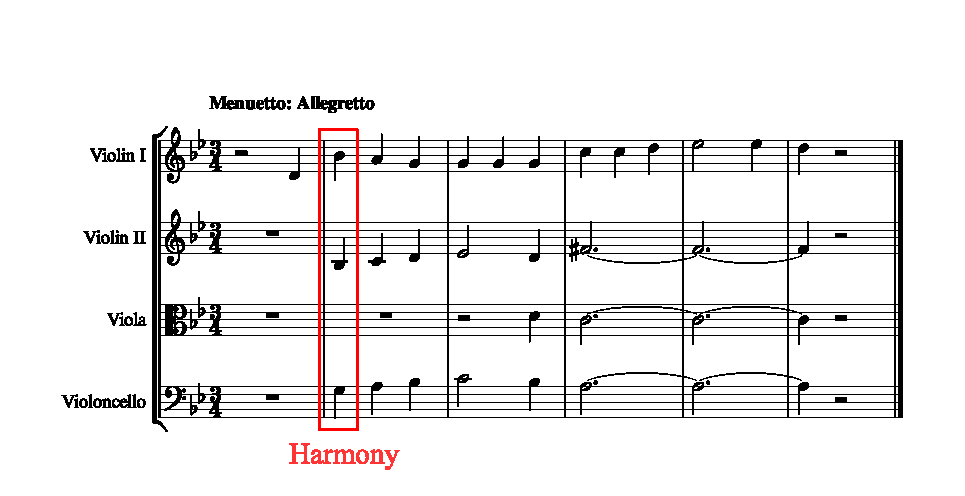
\includegraphics[width=1.0\textwidth]{01-introduction/figures/1}
\end{figure}

Combining these definitions, one possible interpretation of what is a harmonic analysis could be the following:

\begin{quote}
\centering
\emph{[...] the interpretation of \textbf{harmonic} structures in music, \linebreak
their resolution into relatively simpler elements, \textbf{i.e., harmonic labels}, \linebreak and the investigation of the relevant functions of those \textbf{labels}.}
\end{quote}

\begin{figure}[h]
  \caption{Highlighting harmonic structures in musical excerpt}
  \label{fig:harmonic-structures}
  \centering
    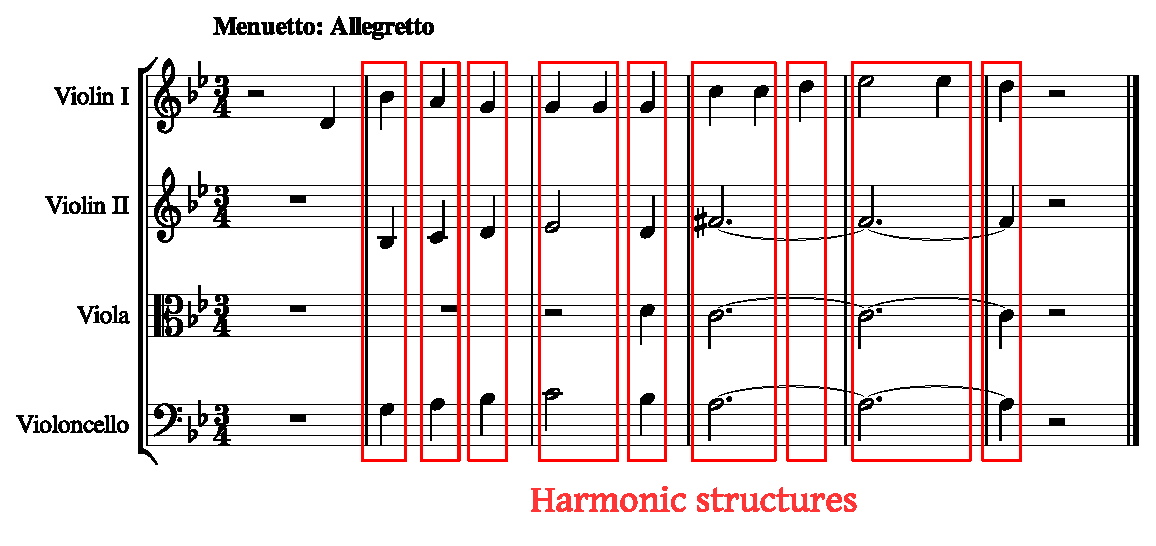
\includegraphics[width=1.0\textwidth]{01-introduction/figures/2}
\end{figure}

Therefore, as stated by this definition, the process of harmonic analysis comprises three steps:

\begin{itemize}
  \item Interpreting the harmonic structures in music
  \item Resolving these harmonic structures into harmonic labels
  \item Investigating the relevant functions among these labels
\end{itemize}

For breaking down the steps of the analysis, we could use a fragment of a musical score. Figure \ref{fig:harmony} remarks the first beat of the second measure, where three instruments play notes together. Every instance of this simultaneities represents harmony. If these harmonies are clustered and interpreted, we come up with harmonic structures, as in Figure \ref{fig:harmonic-structures}

In order to satisfy the second step of harmonic analysis, we could resolve this interpretation of harmonic structures into some sort of simpler representation. Historically, music theorists performing these sort of harmonic analysis will most likely come with a system of labels that represent the meaning of a harmonic structures. There is not a single labeling system for this purpose. Figure \ref{fig:harmonic-labels} shows three possible representations for the harmonic structures of the same music excerpt presented previously.

\begin{figure}[h]
  \caption{Three different harmonic labeling representations of a musical fragment}
  \label{fig:harmonic-labels}
  \centering
    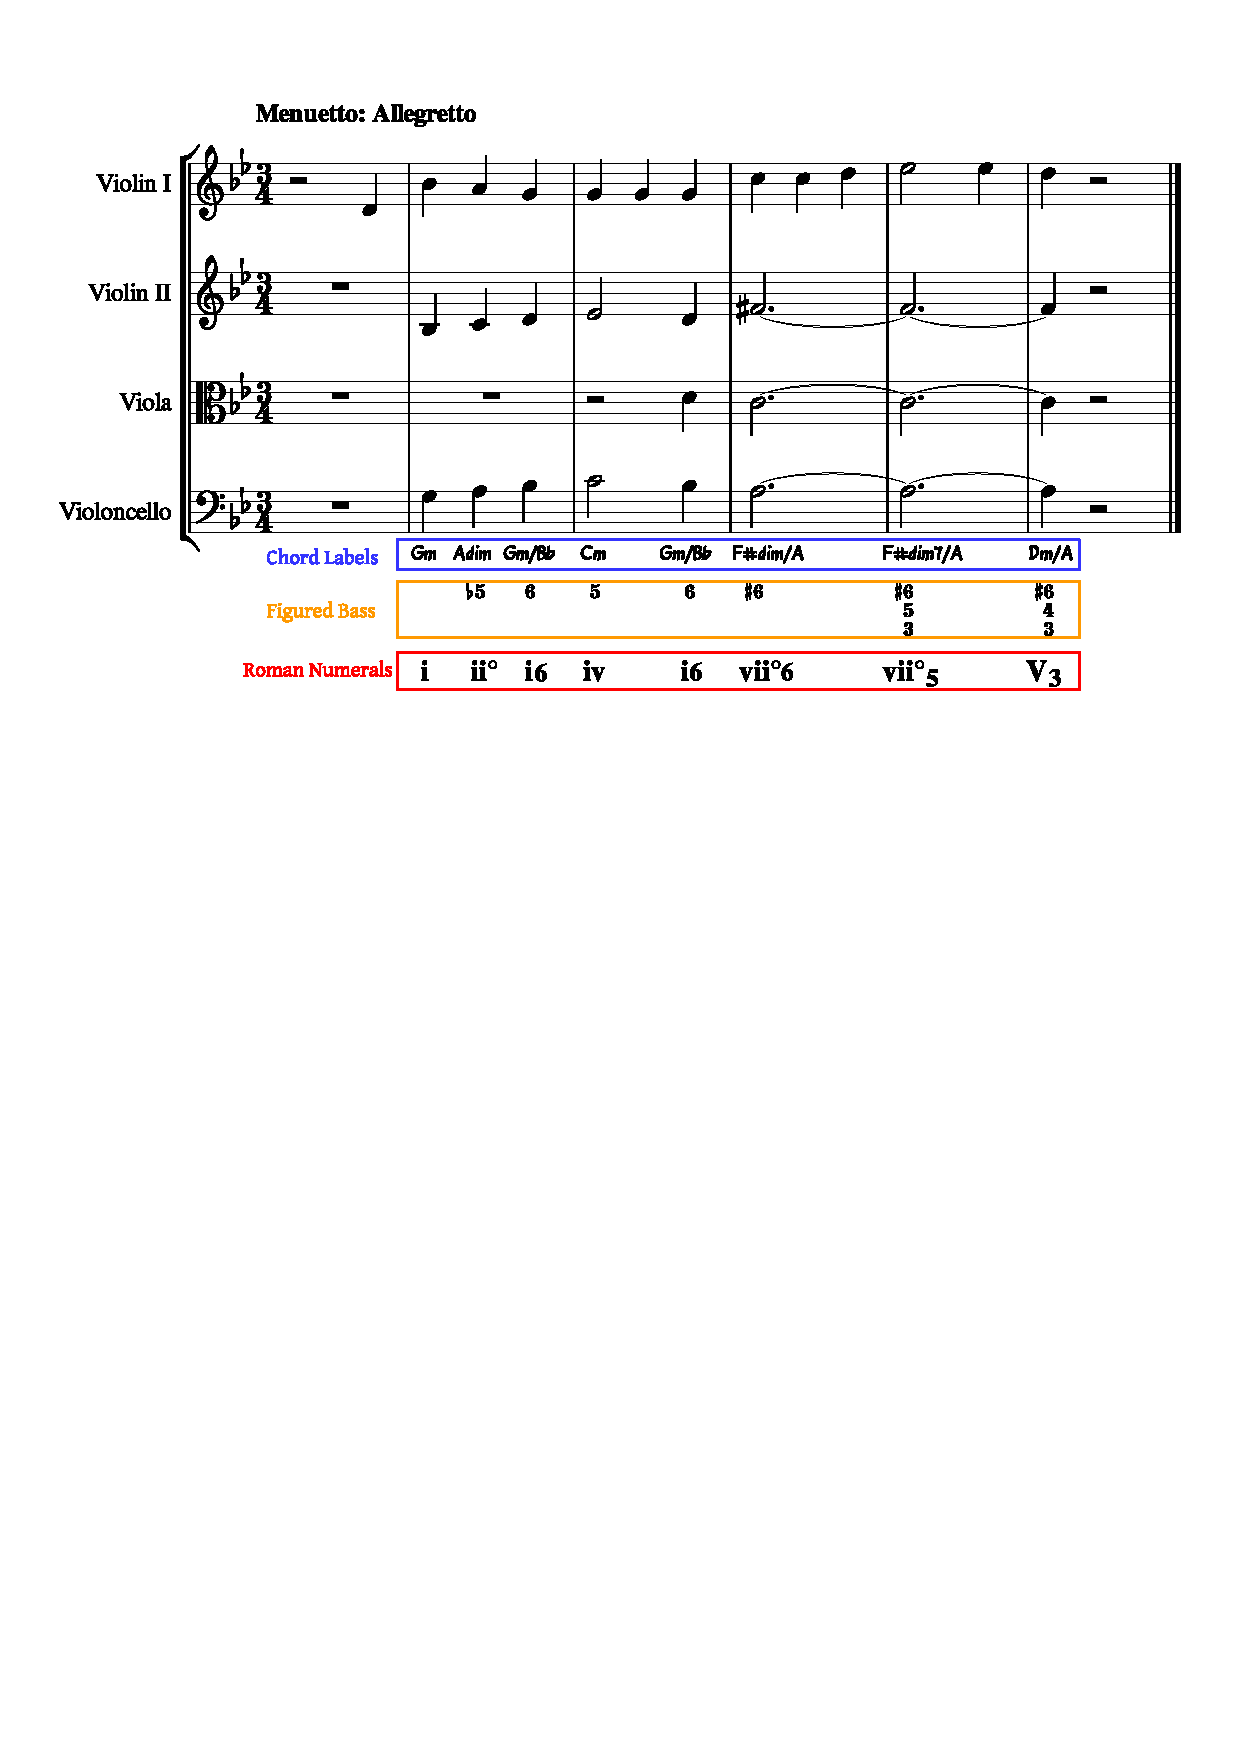
\includegraphics[width=1.0\textwidth]{01-introduction/figures/3}
\end{figure}

Any of these three representations would suffice the second step of harmonic analysis. The chord labels in the first representation are what is commonly seen to label harmonic structures in Jazz and pop music. The figured bass from the second representation was very popular previous to the classical period, and it was intended to aid accompanyists who played in chamber ensembles, e.g., it helped a harpsichordist to "fill-in" the accompaniment during the performance when only one note was given in the score. The third representation using roman numerals emerged previously but consolidated with the theoretical work of Hugo Riemann, and its purpose is mainly of analysis. For this work, I have selected to use the third kind of representation. Further discussion of this harmonic representations is given in the literature review section.

\section{Motivation}
The main reason why it would be benefical for musicians and musicologists to automate a harmonic analysis is because it takes a considerable amount of time and knowledge to perform these analyses. In practice, students at conservatoires often learn the guidelines of harmonic analysis during a specialized course of Harmony. Such a course could extend to several years, making it a difficult discipline to learn fast for a beginner. Even in the case of experts, it might take relatively long time to analyze a piece of music in terms of harmony, which makes the task of automating it valuable even for the expert theorist.

\section{Objectives}
This work pretends to reproduce and apply the current approach for automatic functional harmonic analysis used over the KernScores corpora, and apply it to a specific set of string quartets from Joseph Haydn. Once these automatic analyses are performed, they will be compared to manual annotations over the same set of string quartets.

\section{Structure of the Report}
Literature. Methods. Results. Discussion.

\newpage


% Literature review
\chapter{Literature review}
\section{Harmonic analysis in music theory}
Harmonic analysis could be seen from different perspectives, the first one I would like to address is how it was conceived and modeled by music theorists. Starting with the french composer Jean-Philippe Rameau (1683-1764), until the theory from the german theorist Hugo Riemann (1849-1919) in the late nineteenth century.
  \subsection{Fundamental bass}
  The original idea by Rameau was based on the movement of the bass note, the so called \emph{Fundamental Bass}, which constructed rules and principles of how the movement of a bass note determined also the movement of the harmony. Rameau's theory limited the dictionary of chords to triads and some special cases of seventh chords, and considered chord inversions for the first time, from which the core concept of harmonic root arises and suggests that the bass note could be serving a harmonic root located in the superior voices. This theory is pioneer in separating the melodic movement and coincidence in time from counterpoint \cite{beach1974origins}, and looking at the music from a vertical perspective, a vision that spread in the following periods of western art music.
  \subsection{Root succession tables}
  These set of theories, denomined by Tymoczko as \emph{scale-degree} theories \cite{tymoczko2001root}, assign a number to each of the degrees in a scale, which represents its triad, and then trying to infer the most common succession of that particular scale degree to another. This theories have been used commonly in Harmony text books, and in principle, the scale-degree transitions have not been obtained scientifically. However, due to the probabilistic nature of these theories, there have been recent efforts in validating their statements and accuracy using computational resources, such as first-order Markov models.
  \subsection{Functional harmony}
  In 1893, Hugo Riemann presented his \emph{Vereinfachte Harmonielehre}, which placed together ideas and theories from himself and earlier theorists, and gave birth to what is called \emph{Functional Harmony}. The most notable, and allegedly controversial, characterization that comes from the functions theory, is the idea of categorization of chords. Functional harmony considers that chords belong to one of three tonal functions:
  \begin{itemize}
    \item Tonic
    \item Subdominant
    \item Dominant
  \end{itemize}
  These functions contain all individual chords, but are essentially represented by the primary triads: I, IV and V.
  Due to this categorization of chords, functional harmony contains more information about tonal contexts and semantics, and therefore, as an analysis output becomes more interesting than fundamental bass or root succession theories.
\section{Harmonic analysis in computing}
  Automatic harmonic analysis can be classified in different ways. Most researchers agree that the pioneer work in this problem was the approach from Winograd in 1968 \cite{winograd1968linguistics}.This work is not only important because it is the first and pioneering work in computing a functional harmonic analysis, but also because it linked the computational techniques used in natural language processing to music. Since then, researchers have developed this idea in very different ways. I will discuss first the classical music approaches versus the jazz harmonic analysis approaches. Then I will discuss some of the methods and models used for harmonic analysis problems, which may have quite different purposes in mind. Finally, I will review some of the musicological aspects of the string quartets, Haydn as a composer of classical musical forms, and finally I will discuss the specific string quartet that was manually annotated for this work, its musicological context and so on.
  \subsection{Target musical style}
  Tonal music could comprehend a wide range of music as early baroque's Claudio Monteverdi to 20th century jazz fusion's Allan Holdwsworth. In that sense, an automatic harmonic analysis approach should be able to reach and point out interesting things about all these kinds of music. In practice, however, it is difficult that one approach could serve all sorts of tonal music and at the same time deal with the details, common practices and corner cases from these different music styles and periods. Researchers have systematically split their efforts to target specific kinds of music, and even sometimes, specific composers.
  Among the approaches that cover different kinds of music, there is the General Chord Type (GCT) representation from Emilios Cambouropoulos \cite{cambouropoulos2014idiom}, which is intended to be used in the universal classification of chord verticals according to the idiom that is trying to model. This model is not restricted to tonal music, having the possibility of working in atonal music as well, however, as I stated before, such a flexible model does not deal with the complex and specific scenarios of tonal music, in this case, simply because it is not designed to do it.
  The natural separation that has emerged among researches is to either tackle harmonic analysis targetting classical music or jazz music. As the interest of my work is classical music, I will only briefly describe some of the pillar works in the context of jazz harmonic analysis.
    \subsubsection{Jazz harmonic analysis}
    After Winograd, probably one of the pillar works in harmonic analysis for jazz is that of John Wade Ulrich \cite{ulrich1977analysis}. This work developed a functional analysis, identifying the function of each chord in a musical piece. The input for this model was a sequence of chords and it incorporated the detection of keys. Among some of the restrictions it has is that it does not work for music in a minor tonality, and constraints chord changes to occur once every beat.
    Following to the model from Ulrich, probably one of the next pillars in harmonic analysis oriented to jazz music and a direct successor to the baseline of Ulrich is the model from Francois Pachet \cite{pachet2000computer} who presents a hierarchical model to analyze jazz harmonic progressions, similarly taking as input a sequence of chords and deriving a hierarchical description of modulations. This model does not consider voice-leading and lands in the more "hierarchical" type of analysis, which give structure to a set of chord labels. It was later extended by Ricardo Scholz \cite{scholz2005automating} who attempted to incorporate modal borrowings and secondary dominants.
    From these research, we can infer an important fact, most of the jazz oriented approaches lie within the context of \emph{hierarchical} approaches to functional harmony, and oftenly trivialize the input to chord labels to focus on the functional hierarchies themselves. One of the most important problems in classical music, for example, is precisely in how to deal with all these melodic streams before they can be considered chord labels. This happens maybe because the harmonic movement in Jazz is much more aggressive and departs from a tonal center with ease, making the effort of tracking fast-moving tonal centers an attractive problem, and melodic, polyphonical implications of the music less useful, whereas in classical music it is usual to well-establish one tonal center before moving to the next, at least for the classical period, but extracting the implied tonal function within the different melodic streams is not a trivial task to solve. These characteristics of the music styles probably point out and justify the motivations for separating the models according to the music that is being analyzed.
  \subsection{Type of model}
  Some other way to classify approaches is by the underlying technology used for the analysis
    \subsubsection{Rule-based}
    It is one of the first approaches
    \subsubsection{Probabilistic}

    % Rohrmeier 2008
    This approach also uses MIDI files as input, getting rid of pitch-spelling information, it also seems to be very simplistic as it only extends Melisma in providing major or minor modes for the root analysis. Experiments are done over different kinds of music, which is outside the constraints of classical music that we have set.
    % Rohrmeier 2008

    Most of the rule-based approaches evolved towards probabilistic models. One important example is the Temperley algorithm that is used for this work, which was eventually developed as a Bayesian model in the second version of the Melisma Music Analyzer. However, this has never made out all the way to functional harmonic analysis, that is why I am remaining with the first approach.
    \subsubsection{Grammar-based}
    The first approach, from Winograd is a grammar based approach. Recently, these approaches have been used to find hierarchical relationships between chords.
  \subsection{Target output}
  Probably the most "musical" way of classifying the harmonic analysis, is by the target output the model is expected to produce.
    \subsubsection{Figured bass}
    Barthelemy is the only one.
    \subsubsection{Functional harmonic analysis}
    Winograd, History aside, the input format for the program is not convenient, and as presented by future researchers, the algorithm has problems with certain cases, such as those involving arpeggiations. It cannot be denied that it this work marked a checkpoint and reference for all future work in harmonic analysis.

    Temperley-Sleator-Sapp, Raphael, Illescas

    % Raphael
    This model is one of the few pure-functional harmonic analysis approaches, oriented towards the analysis of common-practice music. The idea is simple and the arbitrary assumptions simplify the parameters of the model. Some constant that remains as in previous models is the fact that it gets rid of all the pitch-spelling information and replaced for solely pitch information. This model, unlike Temperley, does not try to reconstruct the pitch spelling information back by any algorithmic means. I believe this information could be added, and in the words of raphael2003harmonic, it is an obvious extension to the model.
    % / Raphael

    \subsubsection{Tonal hierarchies}
    Rohrmeier, Bas de Haas
\section{String quartets}
  \subsection{Musical form in harmony}
\section{Joseph Haydn}
  \subsection{Who was}
  \subsection{What music does he represent}
  \subsection{His string quartets}
    \subsubsection{Op.20, Sun quartets}

\newpage


% Methodology
\normallinespacing

\chapter{Methods}

\section{Automatic harmonic analysis workflow}
  \subsection{Melisma}
  The Melisma Music Analyzer was implemented by Daniel Sleator over the work of David Temperley. It takes as input a "NoteFile" which is similar to a plain-text representation of midi files.
  In order to achieve a full harmonic analysis, a NoteFile needs to go through 3 stand-alone programs
  	\subsubsection{Meter}
    This program extracts metrical information about the musical piece, using the theories of the Generative Theory of Tonal Music as a basis.
    The output of this program is the same notefile with beat information appended at the end.
    \subsubsection{Harmony}
    This program takes as input the notefile with beat information (the output from the meter program), and outputs information about harmonic roots for each beat. The name is somehow misleading, as this program's output is not harmony, but a harmonic root. Temperley divided the task of harmonic analysis in root estimation and key estimation, this program computing the first of these subtasks. One argument of why they decided to call it "harmony" program instead of "harmonic-root" could be that it was developed before than the key algorithm, and at that moment it was the only analysis done. This information has not been corroborated by me.
    \subsubsection{Key}
    This program takes as input the notefile with beat and harmonic-root information (the ouput from the harmony program). Something to remark about this program is that it might work without the information from the harmony program, estimating only the key, without using any harmonic root information. This could be seen in the following way, if David Temperley divides the problem of harmonic analysis into two subproblems: Root estimation and Key estimation, the first mode of this program pretends to solve the second problem, while in the second mode, adding the output from the "harmony" program as input, pretends to solve both subtasks and output a full harmonic analysis. The difference between these different modes relies on the user setting a certain value in the corresponding parameter file.
    \subsubsection{Parameter files}
    Every program from the Melisma Music Analyzer accepts a parameter file for configuring different options, such as verbosity or roman numeral analysis.
  \subsection{Humdrum extras}
  The humdrum extras are a set of tools developed in C++ by Craig Sapp to process humdrum files (or to convert other formats into humdrum). For this work, we are particularly interested in a few of these utilities that help to process a humdrum file, pass it to the melisma music analyzer, and then bring the output back to humdrum.
   	\subsubsection{Issues with Melisma's input}
    The input format from the Melisma Music Analyzer, yet it resembles a MIDI file, it is not a midi file, and it needs parsing. Humdrum extras provides a parser to convert a humdrum file into the notefile format used by Melisma, this program is called kern2melisma, and it is the first step in the workflow of a functional harmonic analysis from a humdrum score.
    \subsubsection{Piping the output key to key2humdrum}
    Once the file is in Melisma's format, it can go through the melisma programs, as the output of these programs becomes the input for the next one, the files can be piped in unix environment, so it looks like this: kern2melisma | meter | harmony | key.
    At this point, we have the output of the key program from Melisma, this outputs needs additional processing to go back into a humdrum file. There are two programs from Craig Sapp of the MuseInfo tools that enable this process. In this work, I am requiring mainly the key2humdrum program, as this is the one taking the input from the key program, optionally parsing the roman numerals included with the output of the key program.
    \subsubsection{Appending to a humdrum file}
    The last step in getting the information back into a humdrum file is parsing the output of the key2melisma program and appending this information to a humdrum spine. This process is not done by a standalone program, but rather a program that comprehends all the process described before.
    \subsubsection{tsroot summarizes everything}
    The tsroot programs performs all the steps described before, plus interpreting the output of key2humdrum and producing a final humdrum score with the analysis information appended to it.
\section{KernScores}
  \subsection{Content}
  KernScores through its website allows to do an automatic analysis of the scores contained in their corpus.
  \subsection{Automatic analysis using tsroot}
  The website runs the tsroot program over the humdrum scores and show the output to the user.
  \subsection{Op.20 "Sun" quartets}
    19 out of 24 pieces of the Op.20 quartets are contained in KernScores
    \subsubsection{Missing scores}
    The missing scores are:
    \begin{itemize}
      \item Op. 20 No. 1 - III. Affettuoso e sostenuto
      \item Op. 20 No. 2 - II. Capriccio. Adagio
      \item Op. 20 No. 3 - I. Allegro con spirito
      \item Op. 20 No. 4 - I. Allegro di molto
      \item Op. 20 No. 4 - II. Un poco adagio e affettuoso
    \end{itemize}
    \subsubsection{Completing the scores}
    I transcribed these scores manually to complete the set, in some cases using a midi file and hand-fixing it
    \subsubsection{Performed analysis in the website}
    The first thing I did was asking the website to analyze the scores, and reproduce that in my own computer
\section{Dataset}
The dataset consists of 24 pieces, 4900+ chord annotations and commentaries for hard spots.
	\subsection{Manual annotations}
  They follow the **harm syntax
		\subsubsection{**harm syntax}
    It is a valid syntax of the humdrum grammar.
		\subsubsection{**commentary spines}
    Usually located in ambiguous section, or to annotate certain structural analysis (sonata form), but not too methodical.
		\subsubsection{Summary}
    Chords per score?
		\subsubsection{Content}
    All the scores in the dataset
\section{Evaluation}
  \subsection{Evaluation files}
		They are valid Humdrum files with 2 pairs of **harm **root spines
    \subsubsection{Generating}
    Take the manual and automatic, extract the harmonic root using harm2kern, append and filter
    \subsubsection{Rhythmic normalization}
    Files are normalized to the shortest note in the score, specially needed for dealing with polyrhythms
		\subsubsection{Using Humdrum-extras}
    Using harm2kern to extract the harmonic root, for now, that is enough, might change in the future.
	\subsection{Comparing}
		\subsubsection{Resolving root from **harm expression}
    harm2kern for now
		\subsubsection{Ignored annotations}
    Ignoring 'Chr' annotations. See the issues section.
	\subsection{Extracting final results}
		\subsubsection{Total time units}
    The time unit represents the shortest note for that particular score. The scores are normalized to that note as the rhythmic "atom", irrelevant of its value.
		\subsubsection{Percentage}
    Every time unit is matched between manual and automatic file, the percentages are computed considering the total number of "time units" in the score, and the ones that match identically in harmonic root between both files.
		\subsubsection{Distribution of degrees}
    Additional statistics are provided of how the tonal degrees distribute per each score in both, manual and automatic files.
		\subsubsection{Resolution of degree in secondary functions}
    This is a special problem to consider when evaluating functional harmonic analysis. Every subfunction represents a diatonic degree of the current key, an uppercase diatonic degree represents the major mode tonality of that degree, a lowercase diatonic degree represents the minor mode tonality of that degree.
\section{Issues}
This section describes different issues presented and addressed during this work
	\subsection{Transcription issues}
		\subsubsection{Transcription of the missing files from Op.20}
    \begin{itemize}
    \item Op.20 No.4 - I: mm.127
		Replacing E in the first beat of the second violin, for E\#
    \end{itemize}
    \subsubsection{Corrections over the Altmann Edition}
    \begin{itemize}
    \item Op.20 No.2 - I: mm.29
    In the Altmann edition, the bass goes to E flat after a Dominant Seventh chord, however, in other editions it moves to the tonic, it makes more sense to the harmonic context to move towards the tonic, therefore, ignoring the spelling of the Altmann Edition for this measure and considering the bass as heading to the tonic in the third beat of the measure.
    \end{itemize}
		\subsubsection{Corrections over previous KernScores corpus}
    \begin{itemize}
    \item Op.20 No.4 - I: mm.124
    Changing the spelling of the viola from F natural to E sharp as it explains better a dominant seventh chord, and also, it appears like that in the Altmann Edition.

    \item Op.20 No.4 - IV: mm.24
    Adding an e natural to the first violin. It matches what is written in the Altmann Edition, and it makes the harmony clearer, from a g-diminished triad to a fully diminished e natural seventh chord, which explains better the f chord in the next measure

    \item Op.20 No.4 - IV: mm.92 \& mm.94
    Correcting wrong spelling of a note in the viola

    \item Op.20 No.6 - II: mm.5
    Changing the D in the fourth beat of the measure for a B natural, which matches the Altmann Edition
    \end{itemize}
	\subsection{Annotation issues}
    \subsubsection{Corner cases}
      \begin{itemize}
        \item Op.20 No.4 - IV: mm.6
		"The augmented triad on the fifth scale degree may be used as a substitute dominant, and may also be considered as ♭III+,[2] for example in C: V+ = G–B–D\♯, ♭III+ = E♭–G–B♮, and since in every key D\♯ = E♭, they are the same three pitches.", Theories and Practice of Harmonic Analysis. p. 35. ISBN 0-7734-9917-2.
      \end{itemize}
		\subsubsection{Non-expert analysis}
    Most of the analyses were done by me, I am not an expert.
		\subsubsection{Fugues are too contrapunctual}
    The fourth movements of Op.20 No.2, No.5 and No.6 are fugues, these were some of the most difficult scores to analyze, mainly because they are very contrapunctual.
		\subsubsection{Lower quality analysis}
    These two scores were transcribed directly from the manual analysis done in paper, I did not add inversions information neither double-checked the analysis. Extra attention should be put, therefore, as I transcribed directly from the annotations of Rafael Caro. Neither Rafael or I made strict annotations of chord inversion or chord attribute in our manual annotations in pen and paper, however, I was careful trying to annotate this information while transcribing to the harm syntax. I transcribed these last two movements without any judgement of my own in that matter, and I might expect inversion and chord types of these annotations missing. I chose Rafael's annotations because he appeared to be clearer in determining the tonal center of a particular section of music than me, while I tend to refuse to move to mark any modulation unless there is a clear justification, either by harmonic or structural context. Considering the lack of inversions and chord attributes, I believe it is better to have his more verbose annotations in terms of tonal center.
    \begin{itemize}
    \item Op.20 No.5 - I
		\item Op.20 No.6 - I
    \end{itemize}
		\subsubsection{Flat -VII annotated as VII}
    While annotating the scores, I marked the lowered seventh degree of the minor mode simply as VII, while it should be a lowered seventh -VII. It could affect the results.
	\subsection{Workflow issues}
    Lots of issues.
		\subsubsection{Source code coming from different sources}
    The main problem is that the source code comes from different repositories, and it is difficult in terms of reproducibility to put everything together in one place and guarantee it will work.
		\subsubsection{Melisma array sizes}
    There was an "error" in the melisma music analyzer. The size of static structures like arrays, have been hardcoded, in long scores like Op.20 No.3 - I, the program reached buffer overflow and crashed without completing the analysis, I fixed my version of the Melisma Music Analyzer programs to correct this, but this code is not public, as I am not aware of the license of the Melisma source code. If attempting to run the analysis in these files, the programs will crash unless this is fixed.
    \begin{itemize}
    \item Op.20 No.4 - IV
    \item Op.20 No.3 - I
    \item Op.20 No.5- I
    \end{itemize}
		\subsubsection{tsroot harmony2humdrum and key2humdrum}
    tsroot had a different default tempo than kern2melisma, therefore, when running the analysis over files with no explicit tempo information, the result is incorrect. I fixed this in my version of the humdrum extra tools, you can download it from my fork repository. At the moment of this publication, the fix for this has not been merged in the main project repository.
	\subsection{Evaluation issues}
		\subsubsection{Chr chords are ignored}
    I am ignoring the annotations denoted as \emph{Chr} by the automatic analysis, instead of denoting a change of harmony after encountering this tag, I am preserving the previous harmonic root. This is probably wrong and should be addressed in a future evaluation.
		\subsubsection{Resolution of degree in secondary functions}
    Though I described the process to resolve a subfunction, I did not write this code with my harmparser. In practice, I delegated this process to the harm2kern program that is already available in the humdrum extra tools. I did not check if the parser from harm2kern is doing this process as I described it. It might be somewhat different.
	\subsection{Bugfixes}
  As the result of this work, a few problems were addressed
		\subsubsection{tsroot --meldir and --midir args}
    The implementation of tsroot has a hardcoded default value of the meldir and midir directories, when trying to change it with console arguments, the program crashed as there was some issue in the translation of the C string. This problem was detected and now it is corrected in the latest version of humdrum extras. Special thanks to Craig Sapp who double-checked this after I posted in the humdrum forum
		\subsubsection{tsroot tempo correction}
    As stated previously, there is a different default tempo in the tsroot program than the kern2melisma program, this means if a file has not an explicit tempo indication, the output analysis is incorrect. This was the case for the entire dataset of Op.20, so detecting and correcting this issue was crucial for this work. This fix has not been until this point merged into the official humdrum extra repository.
\newpage


% Results
\chapter{Results}

This is an example paragraph. As you can see, the main text uses a font size of 12 pt and a line spacing of 1.5. Neither the paragraphs nor the first lines of paragraphs should be indented.

There is no very strict page limit. Your number of pages will be strongly influenced by the size and total number of your figures and tables. It is recommended staying within 30-50 pages. Do not try to fill as many pages as you can. Longer theses are not necessarily of higher quality and of more non-redundant content than shorter theses. Certainly, a master thesis of 15 pages is too short, and a master thesis of 100 pages is too long.

\section{Tables and graphics}

This is an example paragraph. As you can see, the main text uses a font size of 12 pt and a line spacing of 1.5. Neither the paragraphs nor the first lines of paragraphs should be indented.

There is no very strict page limit. Your number of pages will be strongly influenced by the size and total number of your figures and tables. It is recommended staying within 30-50 pages. Do not try to fill as many pages as you can. Longer theses are not necessarily of higher quality and of more non-redundant content than shorter theses. Certainly, a master thesis of 15 pages is too short, and a master thesis of 100 pages is too long.

 \begin{figure}[!ht]
  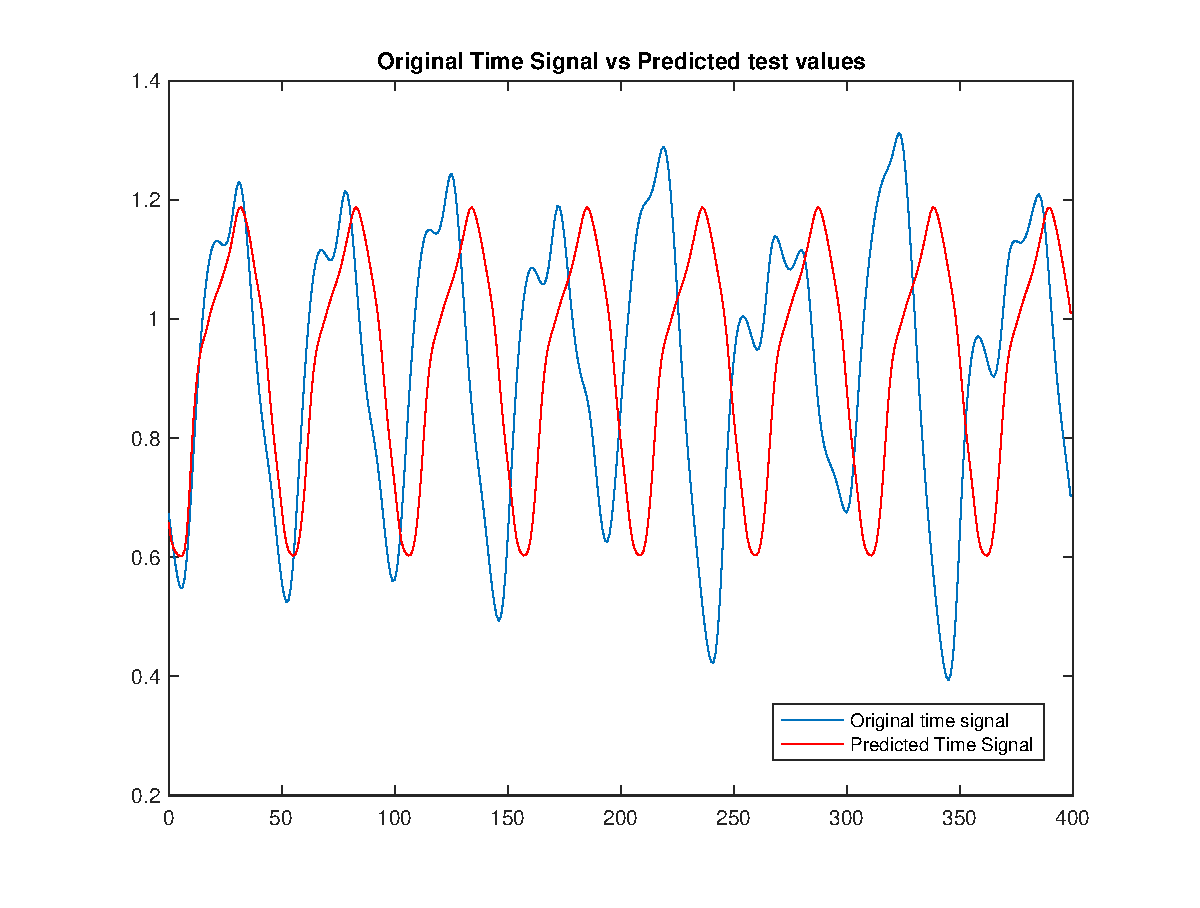
\includegraphics[clip,width=\columnwidth]{Figures/PlotTimeSeriesResult}% 
\caption{This is an example of a figure and its caption.}
\label{fig:timeseries}
\end{figure}

\begin{table}[!ht]
\renewcommand{\arraystretch}{1.50}
\caption{This is an example of a table and its caption.}
\label{tablePCA}
\centering
\begin{tabular}{| c | c |}
\hline
\bfseries PCA & \bfseries Residual mean (in absolute values) \\
\hline\hline
Original PCA & 0.1267  \\
\hline
PCA on Centroid 1 & 0.1249\\
\hline
PCA on Centroid 2 & 0.1214  \\
\hline
\end{tabular}
\end{table}

\newpage




% Conclusion and Discussion
\chapter{Discussion}

\section{Future work}
  \subsection{Musical domain}
    \subsubsection{Beethoven Op.18}
    \subsubsection{Mozart Op.10}
  \subsection{Technological domain}
    \subsubsection{Focusing in scores}
    Leaving cognition behind
    \subsubsection{Pitch-spelling}
    Illescas has done it, but none else

\newpage


\listoffigures
\newpage
\listoftables

% appendices come here
\bibliographystyle{naturemag}
\bibliography{bibliography}

\appendix
\chapter{Issues} %Appendix A
This section describes different issues presented and addressed during this work
	\section{Transcription issues}
		\subsection{Transcription of the missing files from Op.20}
    \begin{itemize}
    \item Op.20 No.4 - I: mm.127
		Replacing E in the first beat of the second violin, for E\#
    \end{itemize}
    \subsection{Corrections over the Altmann Edition}
    \begin{itemize}
    \item Op.20 No.2 - I: mm.29
    In the Altmann edition, the bass goes to E flat after a Dominant Seventh chord, however, in other editions it moves to the tonic, it makes more sense to the harmonic context to move towards the tonic, therefore, ignoring the spelling of the Altmann Edition for this measure and considering the bass as heading to the tonic in the third beat of the measure.
    \end{itemize}
		\subsection{Corrections over previous KernScores corpus}
    \begin{itemize}
    \item Op.20 No.4 - I: mm.124
    Changing the spelling of the viola from F natural to E sharp as it explains better a dominant seventh chord, and also, it appears like that in the Altmann Edition.

    \item Op.20 No.4 - IV: mm.24
    Adding an e natural to the first violin. It matches what is written in the Altmann Edition, and it makes the harmony clearer, from a g-diminished triad to a fully diminished e natural seventh chord, which explains better the f chord in the next measure

    \item Op.20 No.4 - IV: mm.92 \& mm.94
    Correcting wrong spelling of a note in the viola

    \item Op.20 No.6 - II: mm.5
    Changing the D in the fourth beat of the measure for a B natural, which matches the Altmann Edition
    \end{itemize}
	\section{Annotation issues}
    \subsection{Corner cases}
      \begin{itemize}
        \item Op.20 No.4 - IV: mm.6 "The augmented triad on the fifth scale degree may be used as a substitute dominant, and may also be considered as bIII+, for example in C: V+ = G-B-D\#, bIII+ = Eb-G-B, and since in every key D\# = Eb, they are the same three pitches.", Theories and Practice of Harmonic Analysis. p. 35. ISBN 0-7734-9917-2.
      \end{itemize}
		\subsection{Non-expert analysis}
    Most of the analyses were done by me, I am not an expert.
		\subsection{Fugues are too contrapunctual}
    The fourth movements of Op.20 No.2, No.5 and No.6 are fugues, these were some of the most difficult scores to analyze manually, mainly because they are very contrapunctual.
		\subsection{Flat -VII annotated as VII}
    While annotating the scores, I marked the lowered seventh degree of the minor mode simply as VII, while it should be a lowered seventh -VII. It could affect the results.
	\section{Workflow issues}    
		\subsection{Source code coming from different sources}
    The main problem is that the source code comes from different repositories, and it is difficult in terms of reproducibility to put everything together in one place and guarantee it will work.
		\subsection{Melisma array sizes}
    There was an "error" in the melisma music analyzer. The size of static structures like arrays, have been hardcoded, in long scores like Op.20 No.3 - I, the program reached buffer overflow and crashed without completing the analysis, I fixed my version of the Melisma Music Analyzer programs to correct this, but this code is not public, as I am not aware of the license of the Melisma source code. If attempting to run the analysis in these files, the programs will crash unless this is fixed.
    \begin{itemize}
    \item Op.20 No.4 - IV
    \item Op.20 No.3 - I
    \item Op.20 No.5- I
    \end{itemize}
		\subsection{tsroot harmony2humdrum and key2humdrum}
    tsroot had a different default tempo than kern2melisma, therefore, when running the analysis over files with no explicit tempo information, the result is incorrect. I fixed this in my version of the humdrum extra tools, you can download it from my fork repository. At the moment of this publication, the fix for this has not been merged in the main project repository.
	\section{Evaluation issues}
		\subsection{Chr chords are ignored}
    I am ignoring the annotations denoted as \emph{Chr} by the automatic analysis, instead of denoting a change of harmony after encountering this tag, I am preserving the previous harmonic root. This is probably wrong and should be addressed in a future evaluation.
		\subsection{Resolution of degree in secondary functions}
    Though I described the process to resolve a subfunction, I did not write this code with my harmparser. In practice, I delegated this process to the harm2kern program that is already available in the humdrum extra tools. I did not check if the parser from harm2kern is doing this process as I described it. It might be somewhat different.
	\section{Bugfixes}
  As the result of this work, a few problems were addressed
		\subsection{tsroot --meldir and --midir args}
    The implementation of tsroot has a hardcoded default value of the meldir and midir directories, when trying to change it with console arguments, the program crashed as there was some issue in the translation of the C string. This problem was detected and now it is corrected in the latest version of humdrum extras. Special thanks to Craig Sapp who double-checked this after I posted in the humdrum forum
		\subsection{tsroot tempo correction}
    As stated previously, there is a different default tempo in the tsroot program than the kern2melisma program, this means if a file has not an explicit tempo indication, the output analysis is incorrect. This was the case for the entire dataset of Op.20, so detecting and correcting this issue was crucial for this work. This fix has not been until this point merged into the official humdrum extra repository.
\newpage


\end{document}
